% Politecnico di Milano (PoliMi) - School of Industrial and Information Engineering
%
% Last Revision: October 2021
%
% Copyright 2021 Politecnico di Milano, Italy. NC-BY

\documentclass{Configuration_Files/Template}

%------------------------------------------------------------------------------
%	REQUIRED PACKAGES AND  CONFIGURATIONS
%------------------------------------------------------------------------------

% CONFIGURATIONS
\usepackage{parskip} % For paragraph layout
\usepackage{setspace} % For using single or double spacing
\usepackage{emptypage} % To insert empty pages
\usepackage{multicol} % To write in multiple columns (executive summary)
\setlength\columnsep{15pt} % Column separation in executive summary
\setlength\parindent{0pt} % Indentation
\raggedbottom  

% PACKAGES FOR TITLES
\usepackage{titlesec}
% \titlespacing{\section}{left spacing}{before spacing}{after spacing}
\titlespacing{\section}{0pt}{3.3ex}{2ex}
\titlespacing{\subsection}{0pt}{3.3ex}{1.65ex}
\titlespacing{\subsubsection}{0pt}{3.3ex}{1ex}
\usepackage{color}

% PACKAGES FOR LANGUAGE AND FONT
\usepackage[english]{babel} % The document is in English  
\usepackage[utf8]{inputenc} % UTF8 encoding
\usepackage[T1]{fontenc} % Font encoding
\usepackage[11pt]{moresize} % Big fonts

% PACKAGES FOR IMAGES
\usepackage{graphicx}
\usepackage{transparent} % Enables transparent images
\usepackage{eso-pic} % For the background picture on the title page
\usepackage{subfig} % Numbered and caption subfigures using \subfloat.
\usepackage{tikz} % A package for high-quality hand-made figures.
\usetikzlibrary{}
\graphicspath{{./Images/}} % Directory of the images
\usepackage{caption} % Coloured captions
\usepackage{amsthm,thmtools,xcolor} % Coloured "Theorem"
\usepackage{float}

% STANDARD MATH PACKAGES
\usepackage{amsmath}
\usepackage{amsthm}
\usepackage{amssymb}
\usepackage{amsfonts}
\usepackage{bm}
\usepackage[overload]{empheq} % For braced-style systems of equations.
\usepackage{fix-cm} % To override original LaTeX restrictions on sizes

% PACKAGES FOR TABLES
\usepackage{tabularx}
\usepackage{longtable} % Tables that can span several pages
\usepackage{colortbl}

% PACKAGES FOR ALGORITHMS (PSEUDO-CODE)
\usepackage{algorithm}
\usepackage{algorithmic}

% PACKAGES FOR REFERENCES & BIBLIOGRAPHY
\usepackage[colorlinks=true,linkcolor=black,anchorcolor=black,citecolor=black,filecolor=black,menucolor=black,runcolor=black,urlcolor=black]{hyperref} % Adds clickable links at references
\usepackage{cleveref}
\usepackage[square, numbers, sort&compress]{natbib} % Square brackets, citing references with numbers, citations sorted by appearance in the text and compressed
\bibliographystyle{abbrvnat} % You may use a different style adapted to your field

% OTHER PACKAGES
\usepackage{pdfpages} % To include a pdf file
\usepackage{afterpage}
\usepackage{lipsum} % DUMMY PACKAGE
\usepackage{fancyhdr} % For the headers
\fancyhf{}

% Input of configuration file. Do not change config.tex file unless you really know what you are doing. 
% Define blue color typical of polimi
\definecolor{bluepoli}{cmyk}{0.4,0.1,0,0.4}

% Custom theorem environments
\declaretheoremstyle[
  headfont=\color{bluepoli}\normalfont\bfseries,
  bodyfont=\color{black}\normalfont\itshape,
]{colored}

% Set-up caption colors
\captionsetup[figure]{labelfont={color=bluepoli}} % Set colour of the captions
\captionsetup[table]{labelfont={color=bluepoli}} % Set colour of the captions
\captionsetup[algorithm]{labelfont={color=bluepoli}} % Set colour of the captions

\theoremstyle{colored}
\newtheorem{theorem}{Theorem}[chapter]
\newtheorem{proposition}{Proposition}[chapter]

% Enhances the features of the standard "table" and "tabular" environments.
\newcommand\T{\rule{0pt}{2.6ex}}
\newcommand\B{\rule[-1.2ex]{0pt}{0pt}}

% Pseudo-code algorithm descriptions.
\newcounter{algsubstate}
\renewcommand{\thealgsubstate}{\alph{algsubstate}}
\newenvironment{algsubstates}
  {\setcounter{algsubstate}{0}%
   \renewcommand{\STATE}{%
     \stepcounter{algsubstate}%
     \Statex {\small\thealgsubstate:}\space}}
  {}

% New font size
\newcommand\numfontsize{\@setfontsize\Huge{200}{60}}

% Title format: chapter
\titleformat{\chapter}[hang]{
\fontsize{50}{20}\selectfont\bfseries\filright}{\textcolor{bluepoli} \thechapter\hsp\hspace{2mm}\textcolor{bluepoli}{|   }\hsp}{0pt}{\huge\bfseries \textcolor{bluepoli}
}

% Title format: section
\titleformat{\section}
{\color{bluepoli}\normalfont\Large\bfseries}
{\color{bluepoli}\thesection.}{1em}{}

% Title format: subsection
\titleformat{\subsection}
{\color{bluepoli}\normalfont\large\bfseries}
{\color{bluepoli}\thesubsection.}{1em}{}

% Title format: subsubsection
\titleformat{\subsubsection}
{\color{bluepoli}\normalfont\large\bfseries}
{\color{bluepoli}\thesubsubsection.}{1em}{}

% Shortening for setting no horizontal-spacing
\newcommand{\hsp}{\hspace{0pt}}

\makeatletter
% Renewcommand: cleardoublepage including the background pic
\renewcommand*\cleardoublepage{%
  \clearpage\if@twoside\ifodd\c@page\else
  \null
  \AddToShipoutPicture*{\BackgroundPic}
  \thispagestyle{empty}%
  \newpage
  \if@twocolumn\hbox{}\newpage\fi\fi\fi}
\makeatother

%For correctly numbering algorithms
\numberwithin{algorithm}{chapter}

%----------------------------------------------------------------------------
%	NEW COMMANDS DEFINED
%----------------------------------------------------------------------------

% EXAMPLES OF NEW COMMANDS
\newcommand{\bea}{\begin{eqnarray}} % Shortcut for equation arrays
\newcommand{\eea}{\end{eqnarray}}
\newcommand{\e}[1]{\times 10^{#1}}  % Powers of 10 notation

%----------------------------------------------------------------------------
%	ADD YOUR PACKAGES (be careful of package interaction)
%----------------------------------------------------------------------------

\usepackage{geometry}
\usepackage{tabularx}
\usepackage{booktabs,xltabular}

%----------------------------------------------------------------------------
%	ADD YOUR DEFINITIONS AND COMMANDS (be careful of existing commands)
%----------------------------------------------------------------------------

% Set uniform margins
\geometry{
  left=0.8in,
  right=0.8in,
  top=1in,
  bottom=1in,
  includehead,
  includefoot
}

%----------------------------------------------------------------------------
%	BEGIN OF YOUR DOCUMENT
%----------------------------------------------------------------------------

\begin{document}

\fancypagestyle{plain}{%
\fancyhf{} % Clear all header and footer fields
\fancyhead[RO,RE]{\thepage} %RO=right odd, RE=right even
\renewcommand{\headrulewidth}{0pt}
\renewcommand{\footrulewidth}{0pt}}

%----------------------------------------------------------------------------
%	TITLE PAGE
%----------------------------------------------------------------------------

\pagestyle{empty} % No page numbers
\frontmatter % Use roman page numbering style (i, ii, iii, iv...) for the preamble pages

\puttitle{
    title= DD Document,
    name= {Mattia Piccinato, Gabriele Puglisi, Jacopo Piazzalunga},
    academicyear= {2023-24}
 }

%----------------------------------------------------------------------------
%	PREAMBLE PAGES: ABSTRACT (inglese e italiano), EXECUTIVE SUMMARY
%----------------------------------------------------------------------------
\startpreamble
\setcounter{page}{1} % Set page counter to 1

%----------------------------------------------------------------------------
%	LIST OF CONTENTS/FIGURES/TABLES/SYMBOLS
%----------------------------------------------------------------------------

% TABLE OF CONTENTS
\thispagestyle{empty}
\tableofcontents % Table of contents 
\thispagestyle{empty}
\cleardoublepage

%-------------------------------------------------------------------------
%	MAIN TEXT
%-------------------------------------------------------------------------.

\addtocontents{toc}{\vspace{2em}} % Add a gap in the Contents, for aesthetics
\mainmatter % Begin numeric (1,2,3...) page numbering


% FIRST CHAPTER
% --------------------------------------------------------------------------
\chapter{Introduction}

\section{Purpose}

The purpose of the project CodeKataBattle (CKB) is to develop a platform where Students can practice coding together. Educators set up challenges (called Battles) within Tournaments, and Students work in teams to solve them. The platform checks their code automatically, giving scores based on how well it works, how quickly they finish, and how good their code quality is. Educators may optionally give extra scores by checking the work themselves, in a so-called Consolidation Stage which starts right after the end of every Battle. Students get ranked in Tournaments based on their scores obtained in teams, and can earn Badges for some achievements, in order to make learning programming more fun and competitive.

{\color{bluepoli}\rule{\linewidth}{0.1pt}}

\subsection{Goals}

{\color{bluepoli}\rule{\linewidth}{0.1pt}}

\begin{enumerate}
    \item[\textcolor{bluepoli}{G1}] Allows registered Students who enrolled according to the right modalities to participate in a Tournament of Code Kata Battles and take part in its Battles.
    \item[\textcolor{bluepoli}{G2}] Allows registered Educators to manage Tournaments for which they have been granted permission.
    \item[\textcolor{bluepoli}{G3}] Allows registered Students who participate in a Tournament of Code Kata Battles to be rewarded of different achievements.
    \item[\textcolor{bluepoli}{G4}] Allows registered Users to visualize information for which they have granted permission.
    \item[\textcolor{bluepoli}{G5}] Automates code evaluation process using GitHub Actions and some static analysis tools.
\end{enumerate}

{\color{bluepoli}\rule{\linewidth}{0.1pt}}

\section{Scope}

The main features which should be provided in order to achieve the aim of the project are:

\begin{itemize}
\item \textcolor{bluepoli}{Creating Challenges:} Educators can make coding challenges (Battles) that Students can join, alone or in teams (groups), within the context of a Tournament.
\item \textcolor{bluepoli}{Using GitHub Actions for Code Submsissions:} Students are supposed to submit their code for a Battle in their GitHub repository, and the system must be informed of a new commit by a participating Student making use of GitHub Actions.
\item \textcolor{bluepoli}{Checking Code both Automatically and Manually:} The platform assigns a score to Students' code automatically, without the intervention of any Educator. Optionally, Educators may also decide to evaluate the code themselves.
\item \textcolor{bluepoli}{Rankings:} During each Battle, a live ranking of the involved teams is available, enabling participating Students to track their performance. Additionally, live Tournament rankings show how well each Student is performing in the Battles within a given Tournament.
\item \textcolor{bluepoli}{Badges for Achievements:} At the end of every Tournament, Students who achieved good results may be awarded with a special Badges, which are ruled by the Educator who created the Tournament.
\end{itemize}

The main goal is to help Students practice coding, giving them feedback and comparing their results to others.

{\color{bluepoli}\rule{\linewidth}{0.1pt}}

\subsection{Definitions}

{\color{bluepoli}\rule{\linewidth}{0.1pt}}

\begin{itemize}
\item \textcolor{bluepoli}{Battle:} A Code Kata, that is, a challenge in which teams of players need to solve a problem in a specific coding language and submit their code to get a score according to the rules of the Battle.
\item \textcolor{bluepoli}{Tournament:} A competition composed of many Battles in which participants' overall score is the sum of all the scores obtained in every Battle they participated in, individually or in team with other players.
\item \textcolor{bluepoli}{Student:} The User which takes part into the Tournaments of Battles.
\item \textcolor{bluepoli}{Educator:} The User which organizes Tournaments of Battles to which the Students can participate and who manages every aspect about them.
\item \textcolor{bluepoli}{Consolidation stage:} The Consolidation Stage is the phase of a Battle which starts as soon as the submission deadline expires, during which the Educators who manage the Tournament can eventually assign an additional score to every team, which will be summed to the score previously assigned by the platform.
\item \textcolor{bluepoli}{Badge:} A Badge is an achievement marker related to a certain Tournament, obtained by Students if they satisfied the specific conditions defined by the Educator during the creation process of the Tournament.
\end{itemize}

{\color{bluepoli}\rule{\linewidth}{0.1pt}}

\subsection{Acronyms}

{\color{bluepoli}\rule{\linewidth}{0.1pt}}

\begin{itemize}
\item \textcolor{bluepoli}{CK:} Code Kata, that is, a Battle.
\item \textcolor{bluepoli}{CKB:} Code Kata Battle, that is, the name of the platform.
\item \textcolor{bluepoli}{ckbSP:} Code Kata Battle Service Provider.
\item \textcolor{bluepoli}{DMZ:} De-Militarized Zone.
\end{itemize}

{\color{bluepoli}\rule{\linewidth}{0.1pt}}

\subsection{Abbreviations}

{\color{bluepoli}\rule{\linewidth}{0.1pt}}

\begin{itemize}
\item \textcolor{bluepoli}{WPn:} n-th World Phenomena
\item \textcolor{bluepoli}{SPn:} n-th Shared Phenomena
\item \textcolor{bluepoli}{Gn:} n-th Goal
\item \textcolor{bluepoli}{Dn:} n-th Domain Assumption
\item \textcolor{bluepoli}{Rn:} n-th Requirement
\end{itemize}

{\color{bluepoli}\rule{\linewidth}{0.1pt}}

\section{Revision History}

{\color{bluepoli}\rule{\linewidth}{0.1pt}}

\section{Reference Documents}

\begin{itemize}
\item \textcolor{bluepoli}{Assignment document A.Y. 2023/2024}\\
(”Requirement Engineering and Design Project: goal, schedule and rules”)
\item \textcolor{bluepoli}{Software Engineering 2 A.Y. 2023/2024 Slides}\\
(Lecture slides provided during the course)
\end{itemize}

{\color{bluepoli}\rule{\linewidth}{0.1pt}}

\section{Document Structure}

This document is composed of six sections:

\begin{itemize}
\item \textcolor{bluepoli}{1st Chapter:} We begin by presenting the problem statement and outlining the system's objectives. In the scope subsection, we offer insights into the various real-world and shared phenomena that the system addresses. Finally, we provide essential resources for readers, including definitions and abbreviations, to facilitate a comprehensive understanding of this document.
\item \textcolor{bluepoli}{2nd Chapter:} We offer a panoramic view of the system's architecture, starting with a comprehensive overview that articulates the high-level components and their interconnections. Subsequently, it delves into the component view, the deployment view and the runtime view. Furthermore, it details component interfaces, elucidates chosen architectural styles and patterns, and encapsulates additional design decisions made during the system's architectural conception.
\item \textcolor{bluepoli}{3rd Chapter:} We provide an overview of the user interface, as it was presented already in the RASD document.
\item \textcolor{bluepoli}{4th Chapter:} We elucidate the correlation between the delineated requirements in the RASD document and the corresponding design elements articulated in this document, mapping how each requirement aligns with the design components.
\item \textcolor{bluepoli}{5th Chapter:} We delineate the procedural steps and order of operations necessary to bring the design to fruition while ensuring functionality and coherence.
\item \textcolor{bluepoli}{6th Chapter:} We provide an estimate of the effort spent by each group member.
\item \textcolor{bluepoli}{7th Chapter:} We provide a list of the references used in this document.
\end{itemize}

{\color{bluepoli}\rule{\linewidth}{0.1pt}}

% SECOND CHAPTER
% --------------------------------------------------------------------------
\chapter{Overall Description}

The purpose of this section was to present and analyze the architecture of the S2B system in a top- down manner. We first introduced the overall architecture and then provided a diagram of the system’s components, focusing on the ckbSP subcomponent. Next, we used an ER diagram to describe the system’s logical data and presented the system’s deployment view, including the layers and tiers involved. We also used sequence diagrams to depict important runtime views and class diagrams to analyze the component interfaces. Finally, we discussed the architectural design choices and the reasons behind them.

\section{Overview: High-level Components and Interaction}

The figure shown below represents a high-level description of the components which make up the System. In this document the presentation layer and the Client (e.g. the Browser) will be referred to as the Frontend, while the Application Layer and the Data Layer will be referred to as the Backend.

\begin{figure}[H]
\centering
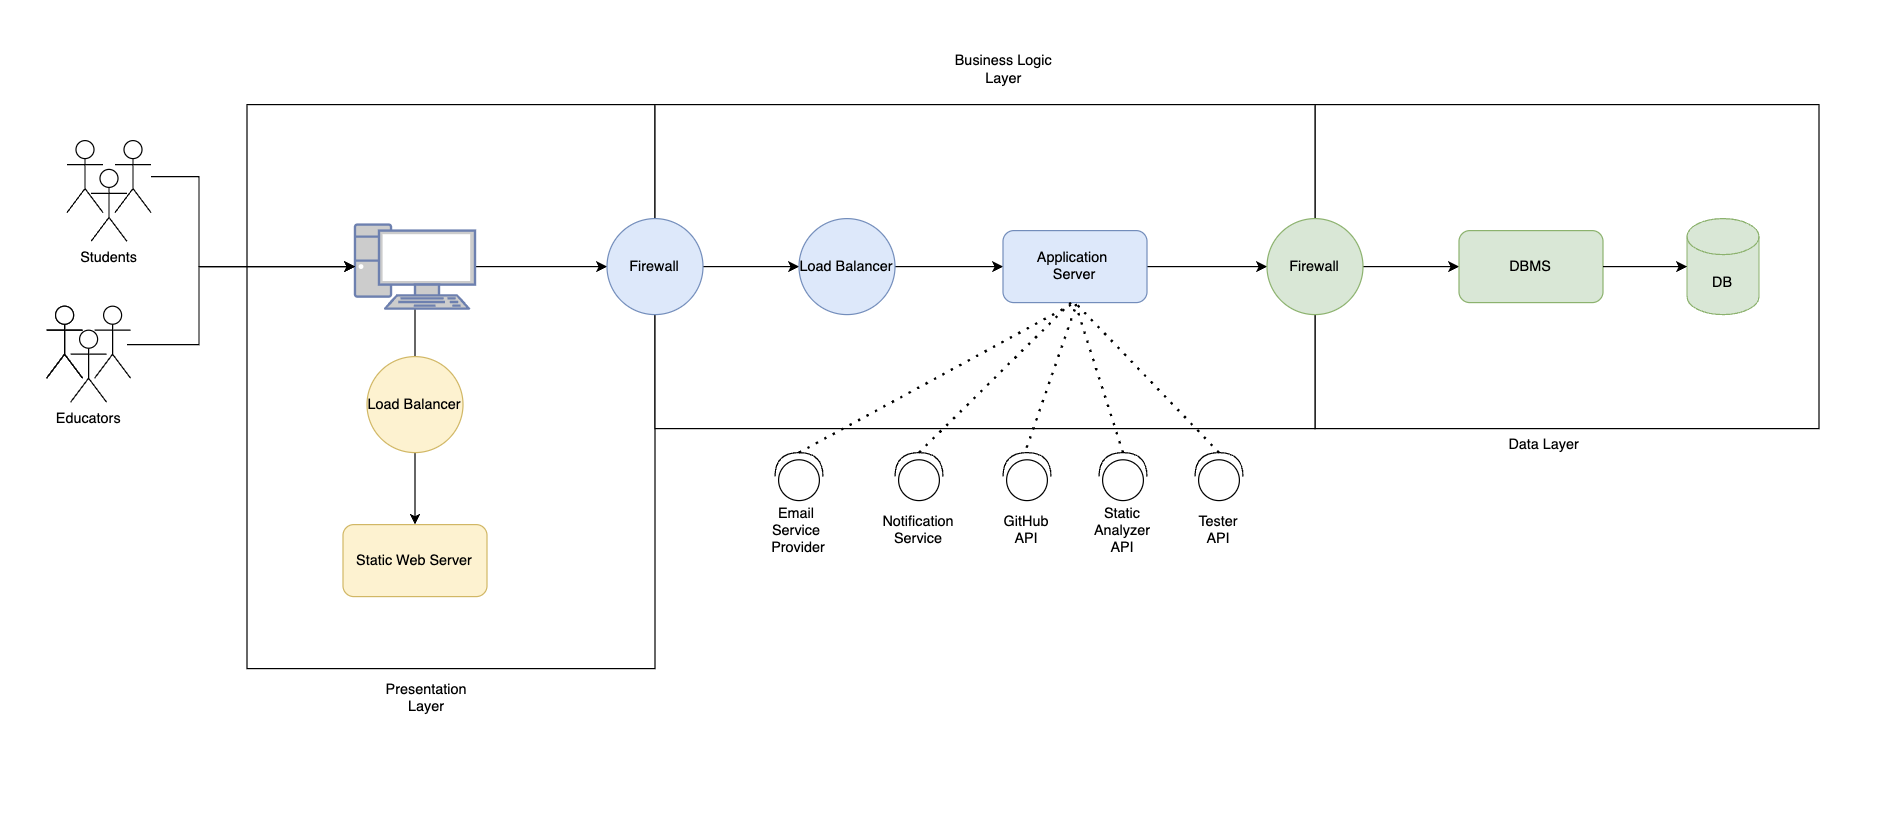
\includegraphics[scale = 0.5]{DD_latex/Images/diagrams/overview.png}\\
\end{figure}


A web interface will be used to access the service. A single page application (SPA) will be developed for educators and students to use the system. An SPA is a good choice for this type of application because it allows for a lot of interaction without the need for frequent page reloads, which can provide a faster and more seamless user experience. The overall architecture of the system is divided into different layers, with the application servers interacting with a database management system and using APIs to retrieve and store data. The application servers are designed to be stateless according to REST standards, and the system includes firewalls to enhance security.

{\color{bluepoli}\rule{\linewidth}{0.1pt}}

\section{Component View}

In this section we show the components of the S2B and their relationships. The following sections will explain the interaction between interfaces and details on each method of interfaces with REST endpoints, if any.

\begin{figure}[H]
\centering
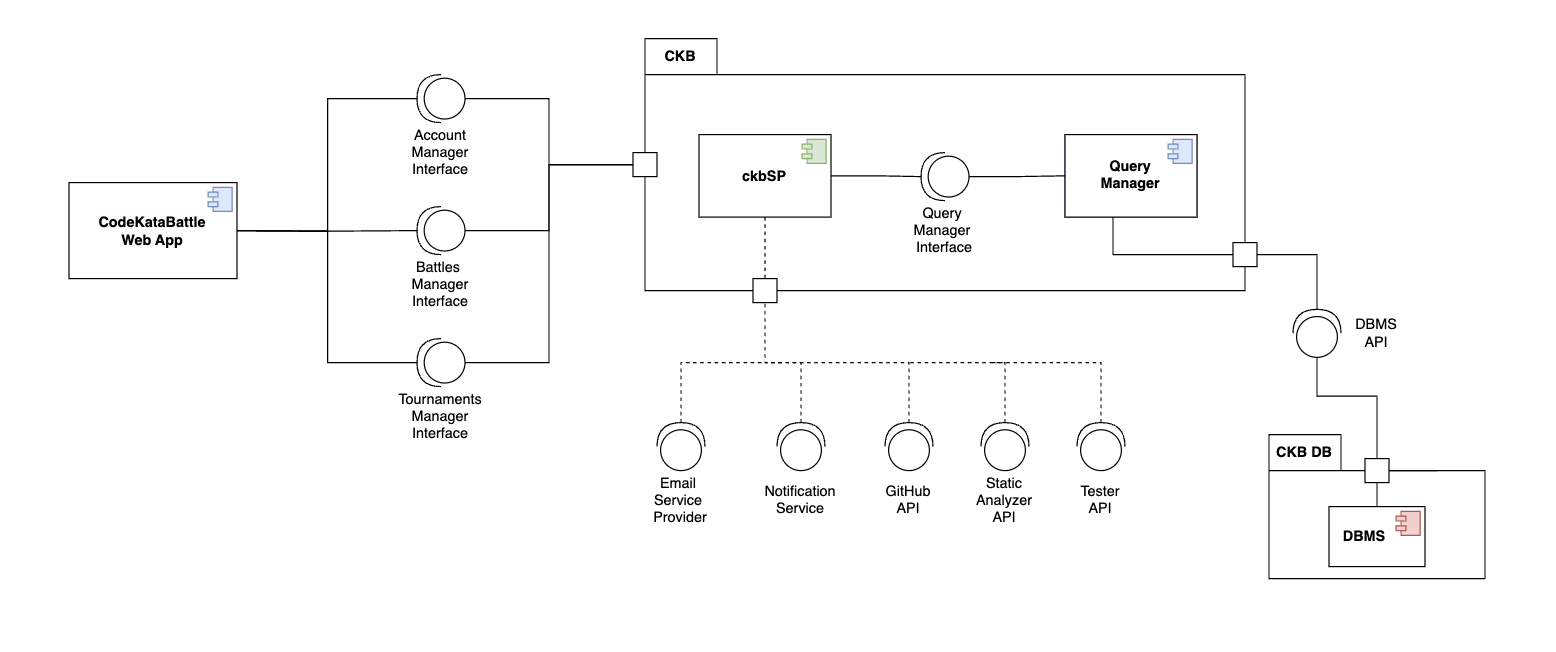
\includegraphics[scale = 0.6]{DD_latex/Images/diagrams/Component_view.png}\\
\caption{Component Diagram of the CodeKataBattle System}
\end{figure}

\subsection{Query Manager}

This component is responsible for communication with a Database Management System (DBMS). It follows the Adapter design pattern, allowing other components to interact with the DBMS without needing to write any SQL code themselves.

\subsection{ckbSP}

The ckbSP subsystem implements CKB's logic. It provides all the system's features, interacting with the other components.

\begin{figure}[H]
\centering
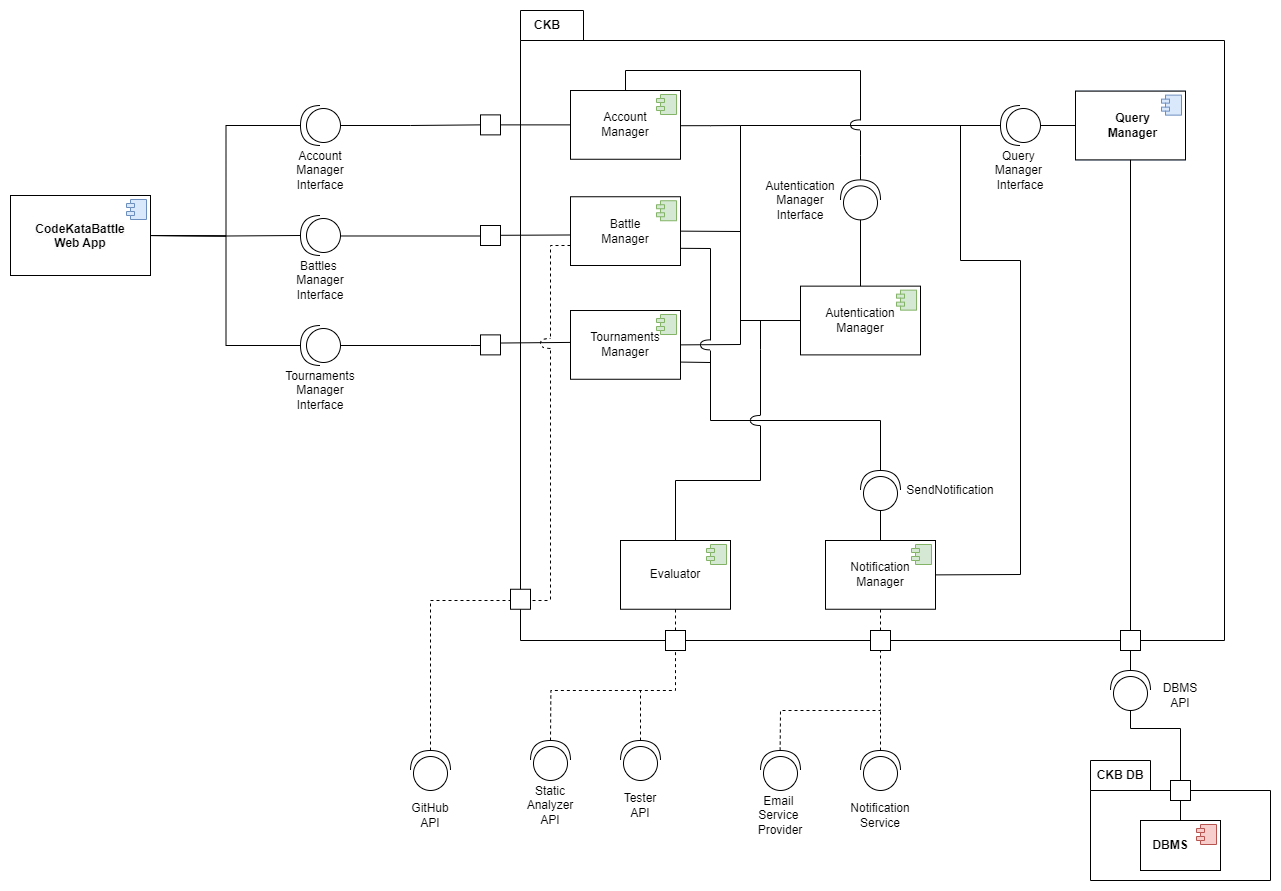
\includegraphics[scale = 0.6]{DD_latex/Images/diagrams/ComponentViewCKBSP.png}\\
\caption{Component Diagram of the ckbSP subsystem}
\end{figure}

\begin{enumerate}
  \item \textcolor{bluepoli}{Account Manager} This component handles the operations needed to manage each User's account, and to view the Students' profiles. It allows Users to login, using the Authentication Manager's interface.
    \item \textcolor{bluepoli}{Battle Manager} This component handles the operations needed to manage a Battle, to view any information about it and to subscribe.
    \item \textcolor{bluepoli}{Tournament Manager} This component handles the operations needed to manage a Tournament, to view any information about it and to subscribe.
    \item \textcolor{bluepoli}{Autentication Manager} This component handles signup, login and logout operations.
    \item \textcolor{bluepoli}{Evaluator} This component is responsible for automatically computing the score of Students' code when a commit is performed. 
    \item \textcolor{bluepoli}{Notification Manager} This component is responsible for the notification dispatch.
\end{enumerate}

\subsection{Logical Description of Data}

In this section the ER diagram of CKB's data is shown. An ER diagram is a graphical representation of the structure of a database, showing the relationships between entities and their attributes.

\begin{figure}[H]
\centering
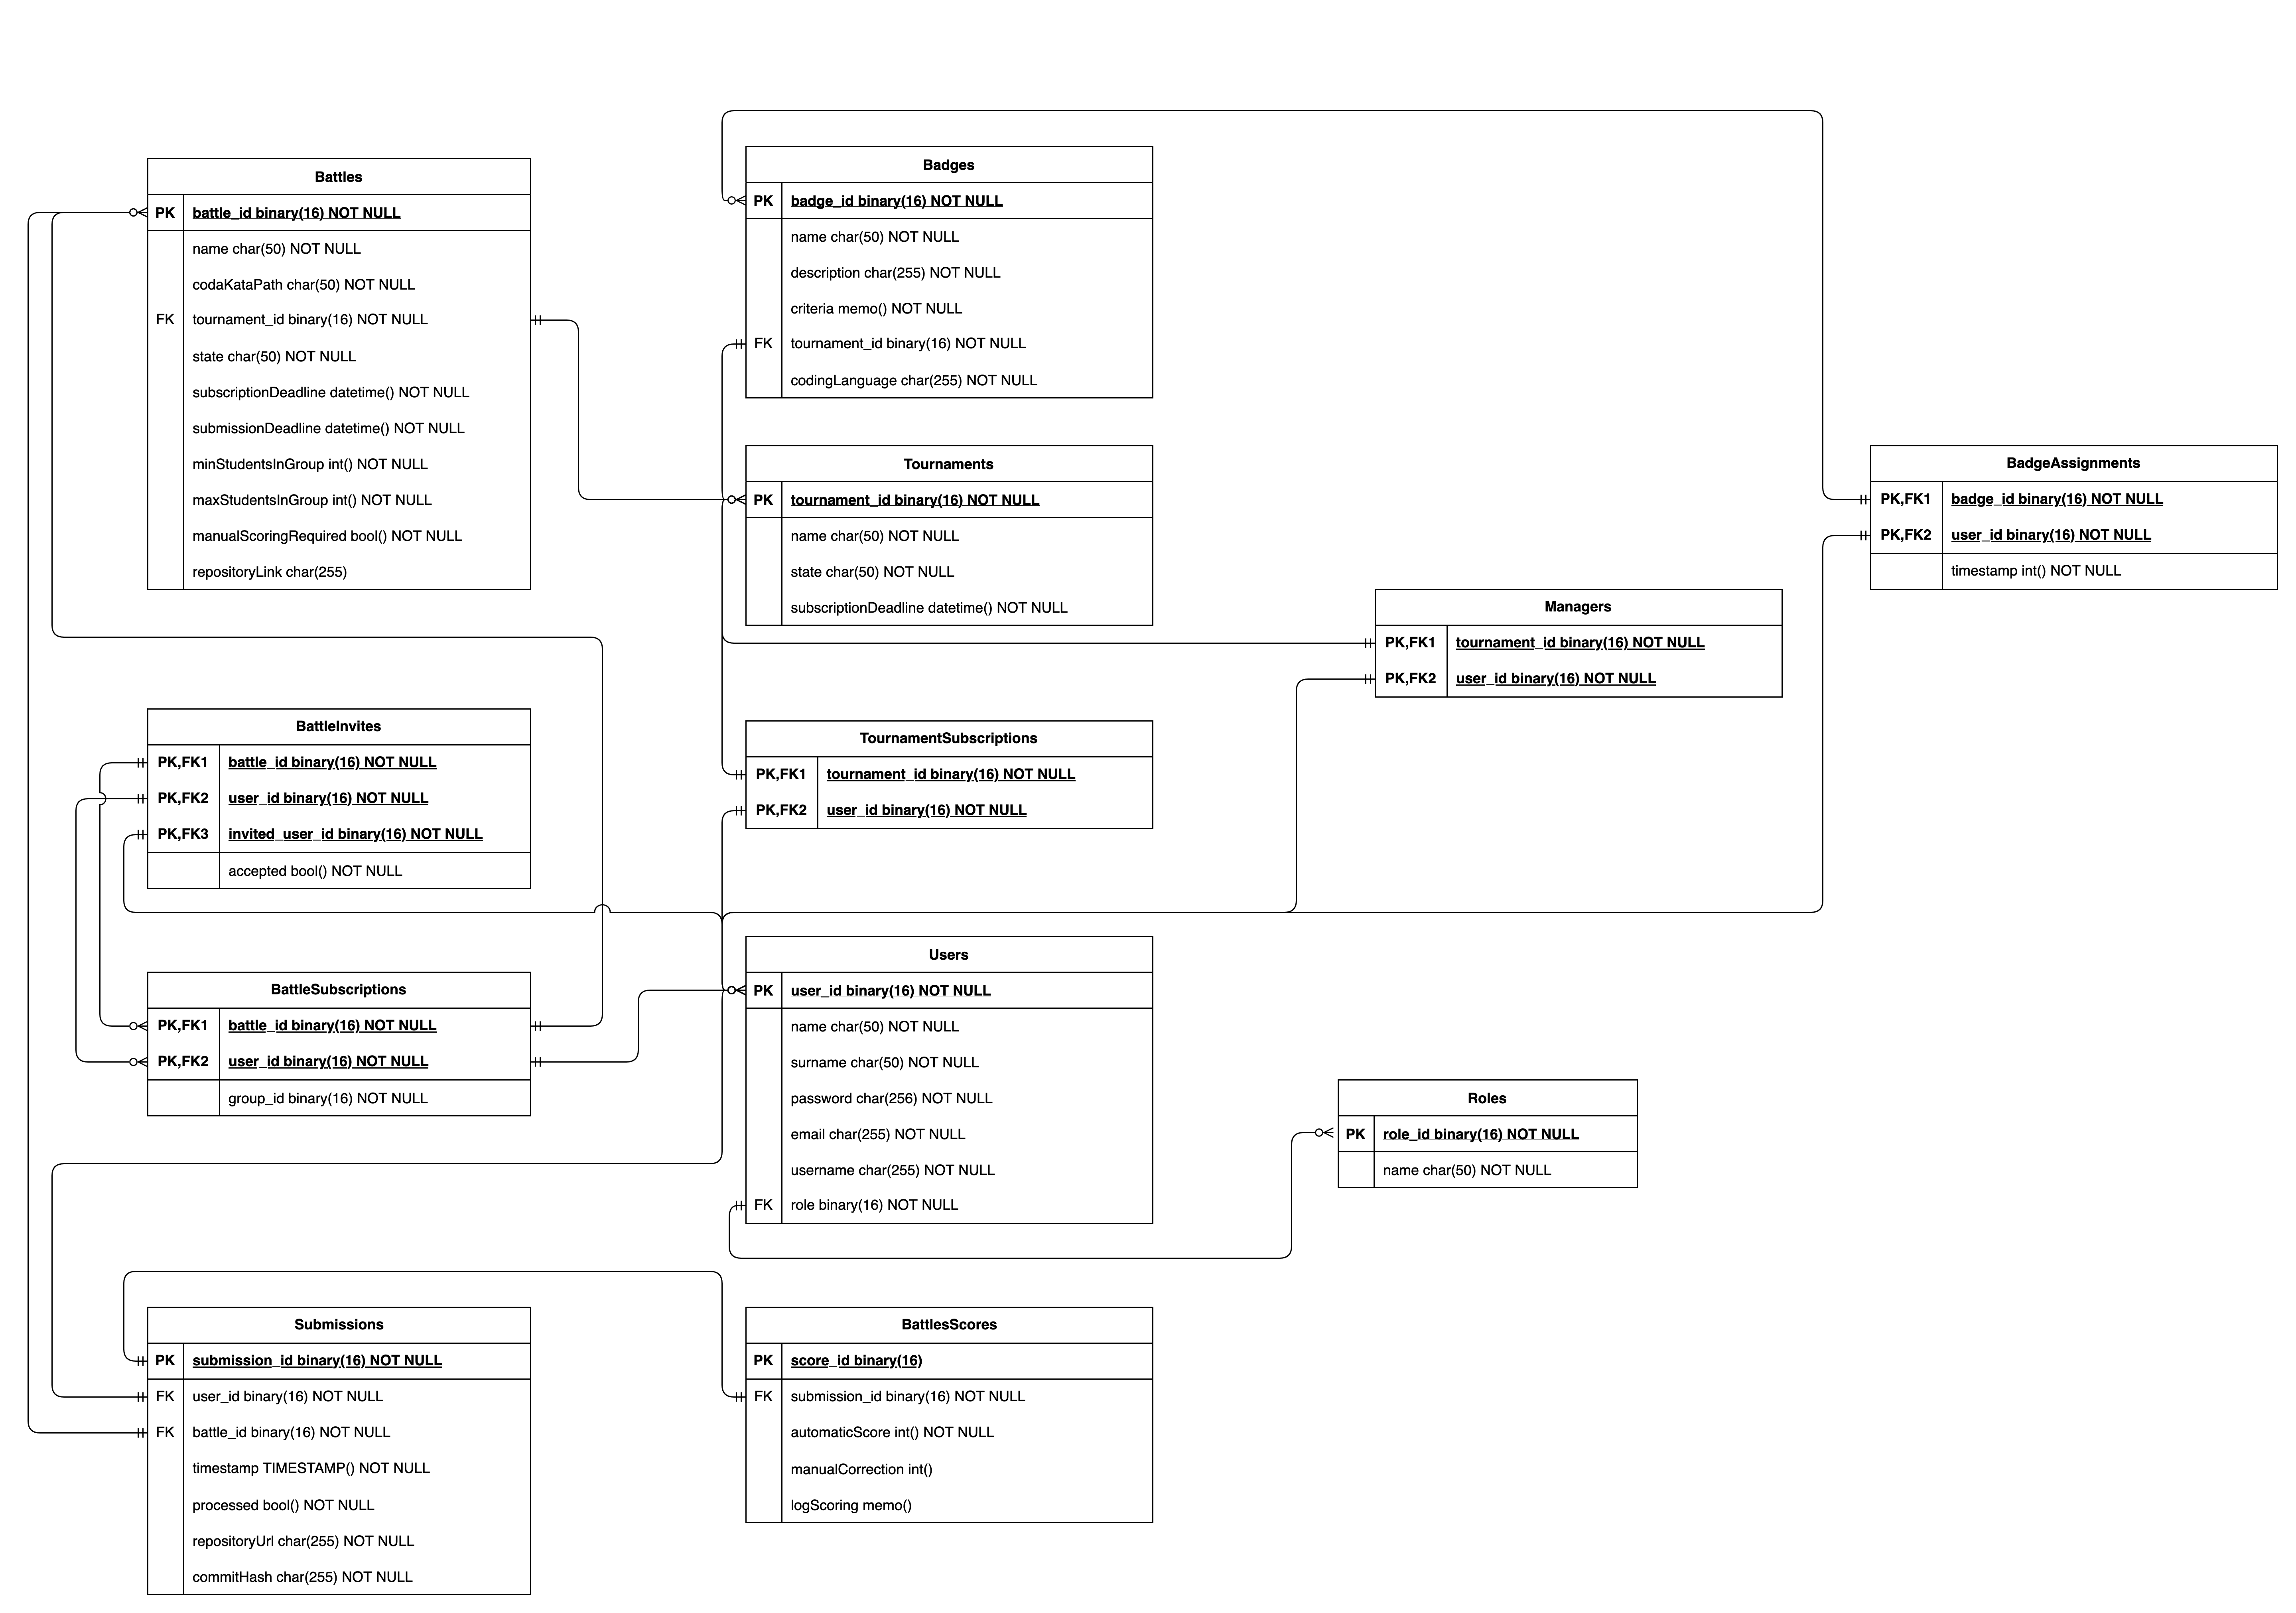
\includegraphics[scale = 0.3]{DD_latex/Images/diagrams/ER_Diagram.png}\\
\caption{ER Diagram of the ckbSP subsystem}
\end{figure}

Additional constraints and triggers must be established in the database management system to ensure data coherence and consistency.

When a battle deadline is reached and its status changes, a trigger should be implemented. This trigger will verify that each group meets the minimum required number of Students. Groups failing to meet this requirement will be automatically unsubscribed from the Battle.

Furthermore, constraints are necessary to maintain role-specific restrictions. Educators must not be included in Battle subscriptions and invitations, and students should not be allowed to manage Tournaments.

Another important constraint is to prevent Users from being enrolled in the same Battle under different groups. This combination of triggers and constraints is crucial for upholding data integrity and consistency in the system.

{\color{bluepoli}\rule{\linewidth}{0.1pt}}

\section{Deployment View}

The system adopts a robust 3-tier architecture hosted on cloud infrastructure, meticulously designed to optimize performance, scalability, and security.

The entire architecture is hosted on a cloud provider. This offers several advantages compared to traditional in-house hosting, such as:
\begin{enumerate}
\item Scalability and Flexibility - the ability to add or remove resources such as virtual machines, performance cores, or memory as needed, and the use of load balancing services, allows the servers to adapt to changes in traffic or workload.
\item Security - services like live monitoring and firewalls help to protect the application server against data breaches and other security threats.
\item Cost-efficiency - the pay-as-you-go model of a cloud provider allows to only pay for the resources that are actually used, which can help to lower the overall costs.
\end{enumerate}
These features make a cloud provider an ideal choice for hosting large, high-traffic applications. The chosen cloud provider will need to offer all of these features in order to meet our needs.

The web server resides in the DMZ and functions as the primary interface for user interaction, managing HTTP requests and delivering web pages. The application server executes the core application logic, processing user requests and handling business operations. Load balancers are implemented to evenly distribute incoming traffic across multiple instances of Web and Application Servers.

\begin{figure}[H]
\centering
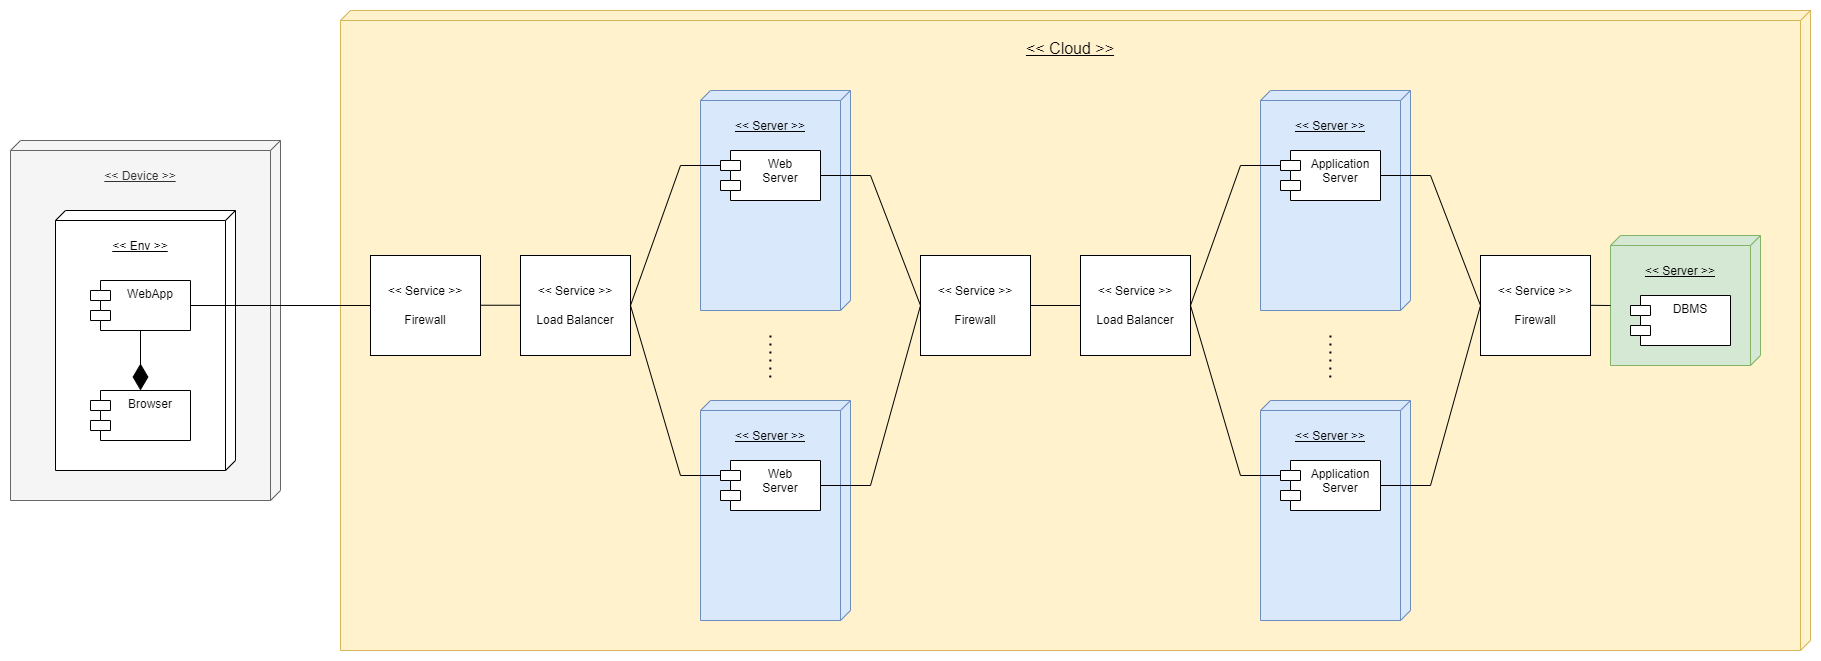
\includegraphics[scale = 0.4]{DD_latex/Images/diagrams/Deployment_view.png}\\
\caption{Component Diagram of the ckbSP subsystem}
\end{figure}

{\color{bluepoli}\rule{\linewidth}{0.1pt}}

\section{Runtime View}

{\color{bluepoli}\rule{\linewidth}{0.1pt}}

\section{Component Interfaces}

{\color{bluepoli}\rule{\linewidth}{0.1pt}}

\section{Selected Architectural Styles and Patterns}

\begin{enumerate}
    \item \textcolor{bluepoli}{Three-Tier} The 3-tier architecture divides the system into three logical layers: presentation (Web Server), business logic (Application Server), and data storage (Database). Each tier has specific functions, ensuring separation of concerns and efficient management of the system. It allows scalability, simplifies maintenance and enhancing control and security. 
    \item \textcolor{bluepoli}{RESTful APIs} RESTful APIs (Representational State Transfer) follow a design paradigm based on specific principles for creating web services. They use standard HTTP methods (GET, POST, PUT, DELETE) and are stateless, allowing easy data exchange between systems. It provides seamless integration with various platforms and systems, it is simple to implement and reduces server load.
    \item \textcolor{bluepoli}{On-Cloud} The system is hosted on cloud infrastructure, leveraging services provided by any cloud provider. This offers on-demand scalability, cost efficiency and ensures high availability.
\end{enumerate}

{\color{bluepoli}\rule{\linewidth}{0.1pt}}

\section{Other Design Decisions}

\subsection{Scale-out} 

The decision to implement a scale out design in the software was taken to enhance its ability to scale, its availability, and its performance. This design approach enables the system to expand its capacity to cope with increased demand by adding more resources, such as servers or machines, as needed. This can be more cost-effective than upgrading individual components and avoids the need for downtime. The scale out design also improves the system’s reliability by providing redundant resources that can take over if
any component fails. In addition, the design allows for flexibility, as resources can be added or removed as required. Lastly, the scale out design improves the system’s performance by allowing workloads to be processed in parallel rather than sequentially.

\subsection{Relational Database}

We selected a relational database for our system design because it is effective at storing structured data, enforcing data integrity, and providing fast query performance. It can also scale to handle large amounts of data and support many concurrent users. The database allows us to store and retrieve information efficiently, while also ensuring that the data is accurate and consistent.
{\color{bluepoli}\rule{\linewidth}{0.1pt}}

\section{Other Design Decisions}

{\color{bluepoli}\rule{\linewidth}{0.1pt}}


% THIRD CHAPTER
% --------------------------------------------------------------------------
\chapter{User Interface Design}

{\color{bluepoli}\rule{\linewidth}{0.1pt}}

\begin{figure}[H]
\centering
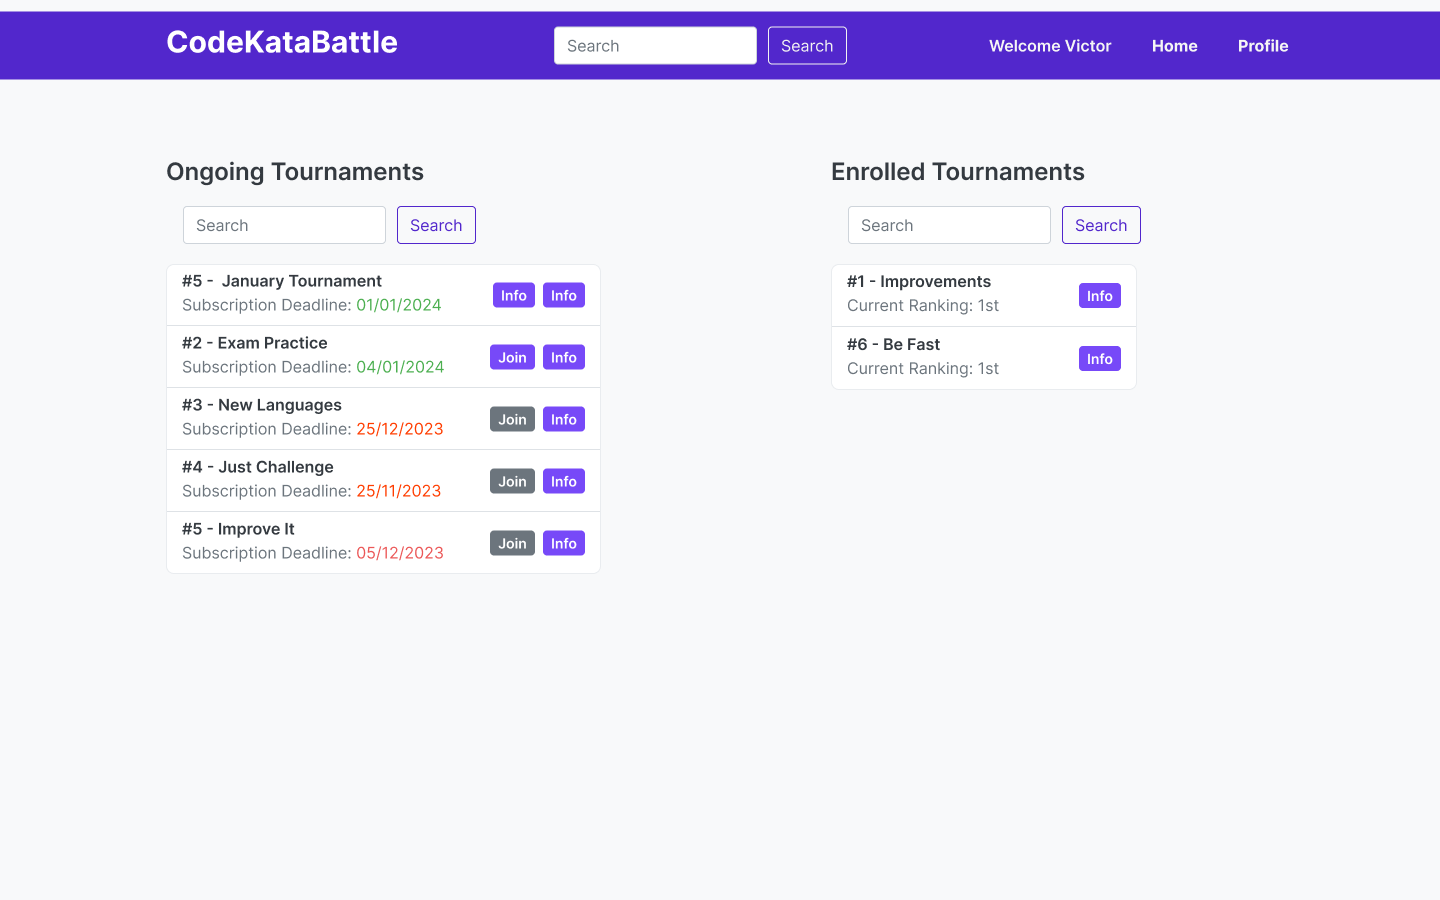
\includegraphics[scale = 0.25]{DD_latex/Images/UI/MainPage_Student.png}\\
\caption{Home Page (Student)}
\end{figure}

\begin{figure}[H]
\centering
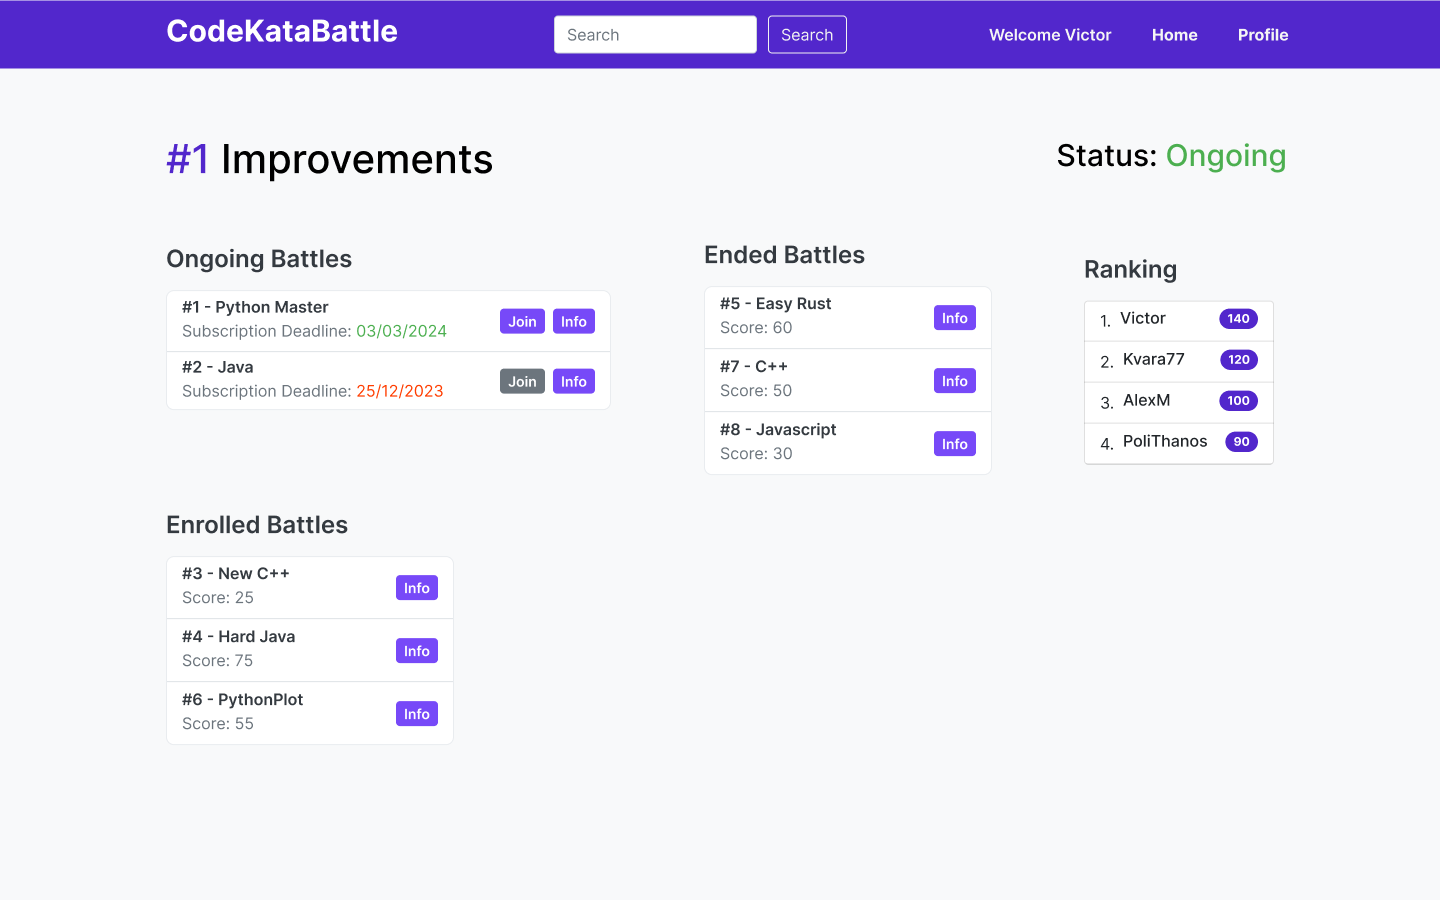
\includegraphics[scale = 0.25]{DD_latex/Images/UI/TournamentPage_Student.png}\\
\caption{Tournament Page (Student)}
\end{figure}

\begin{figure}[H]
\centering
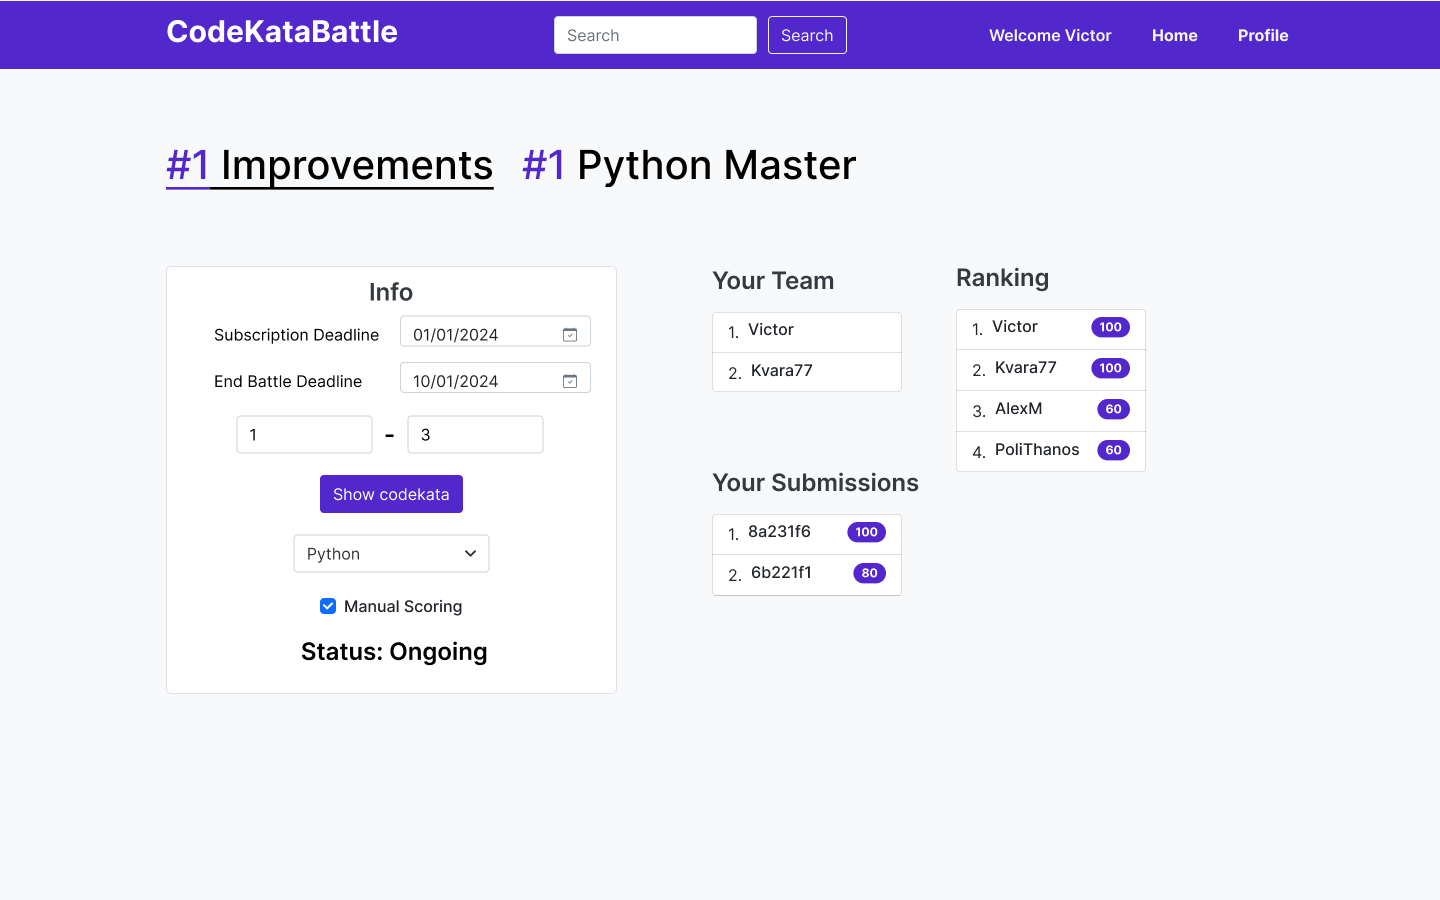
\includegraphics[scale = 0.25]{DD_latex/Images/UI/BattlePage_Student.png}\\
\caption{Battle Page (Student)}
\end{figure}

\begin{figure}[H]
\centering
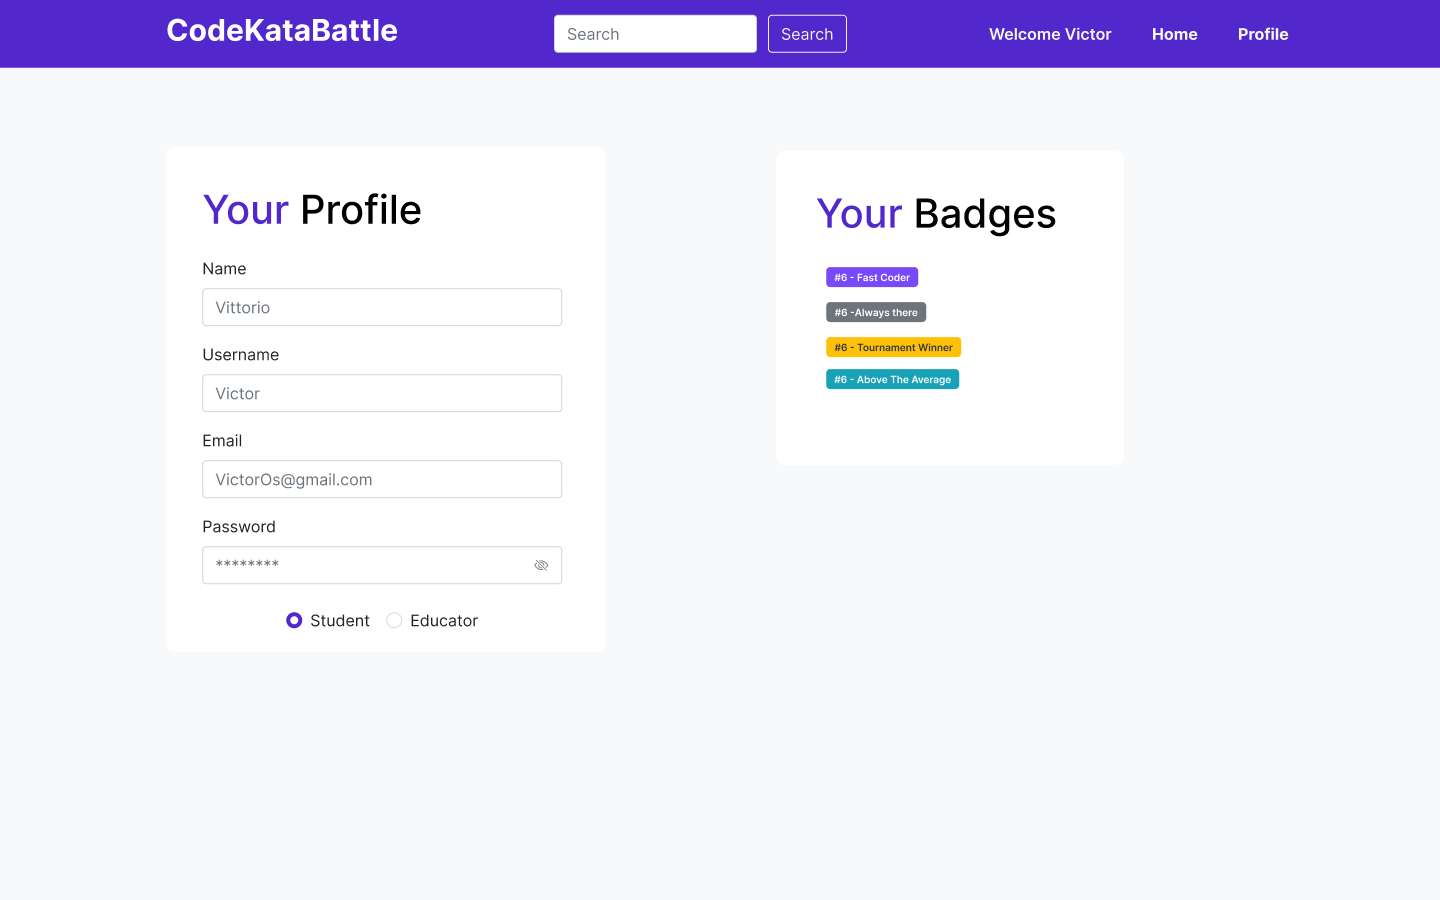
\includegraphics[scale = 0.25]{DD_latex/Images/UI/Profile_Student.png}\\
\caption{Profile Page (Student) }
\end{figure}

\begin{figure}[H]
\centering
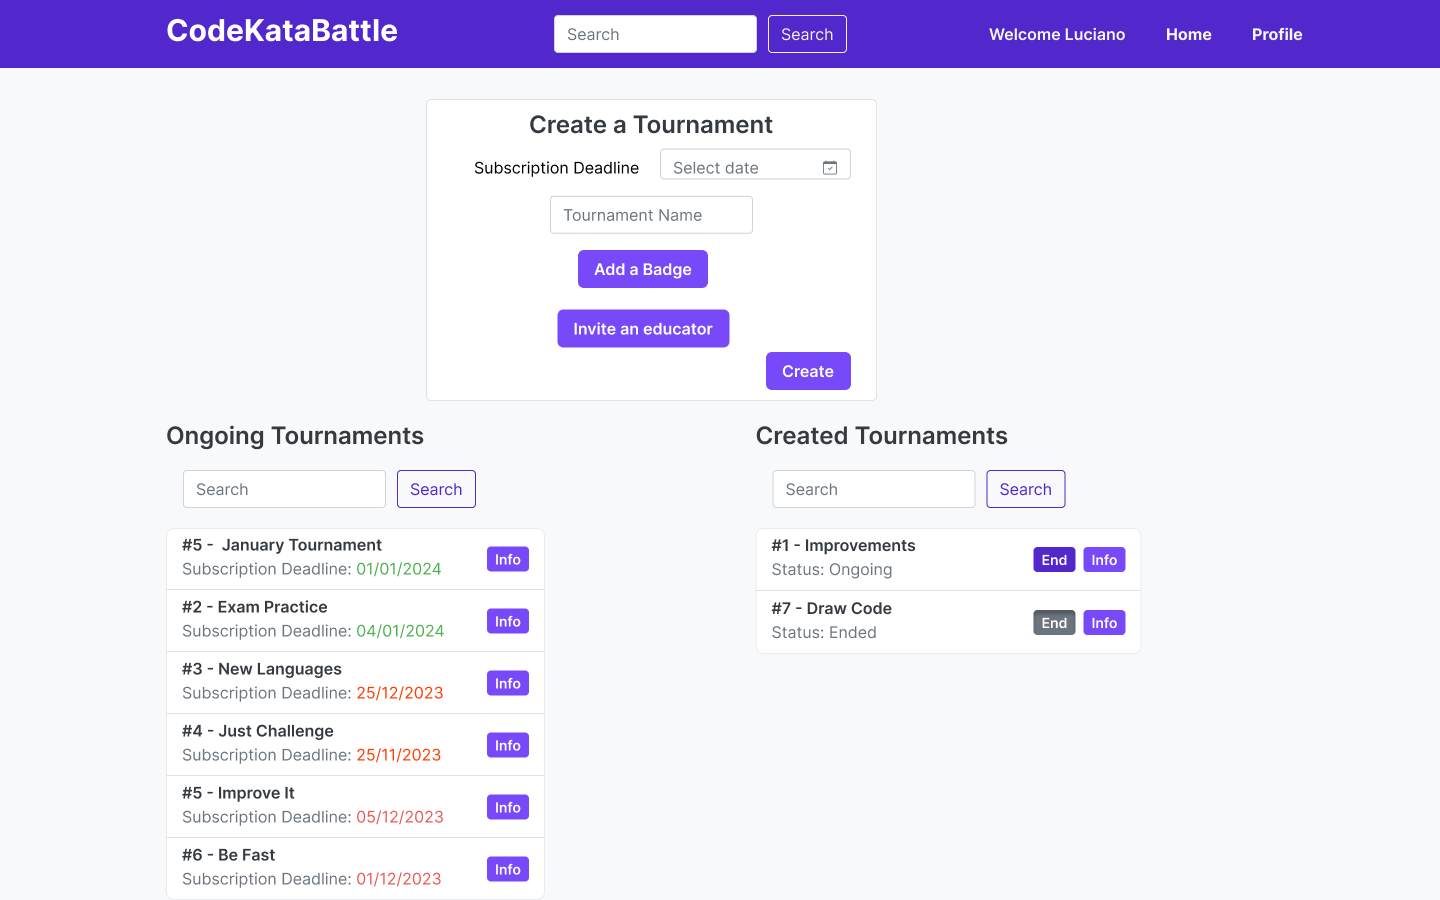
\includegraphics[scale = 0.25]{DD_latex/Images/UI/MainPageEducator.png}\\
\caption{Home Page (Educator)}
\end{figure}

\begin{figure}[H]
\centering
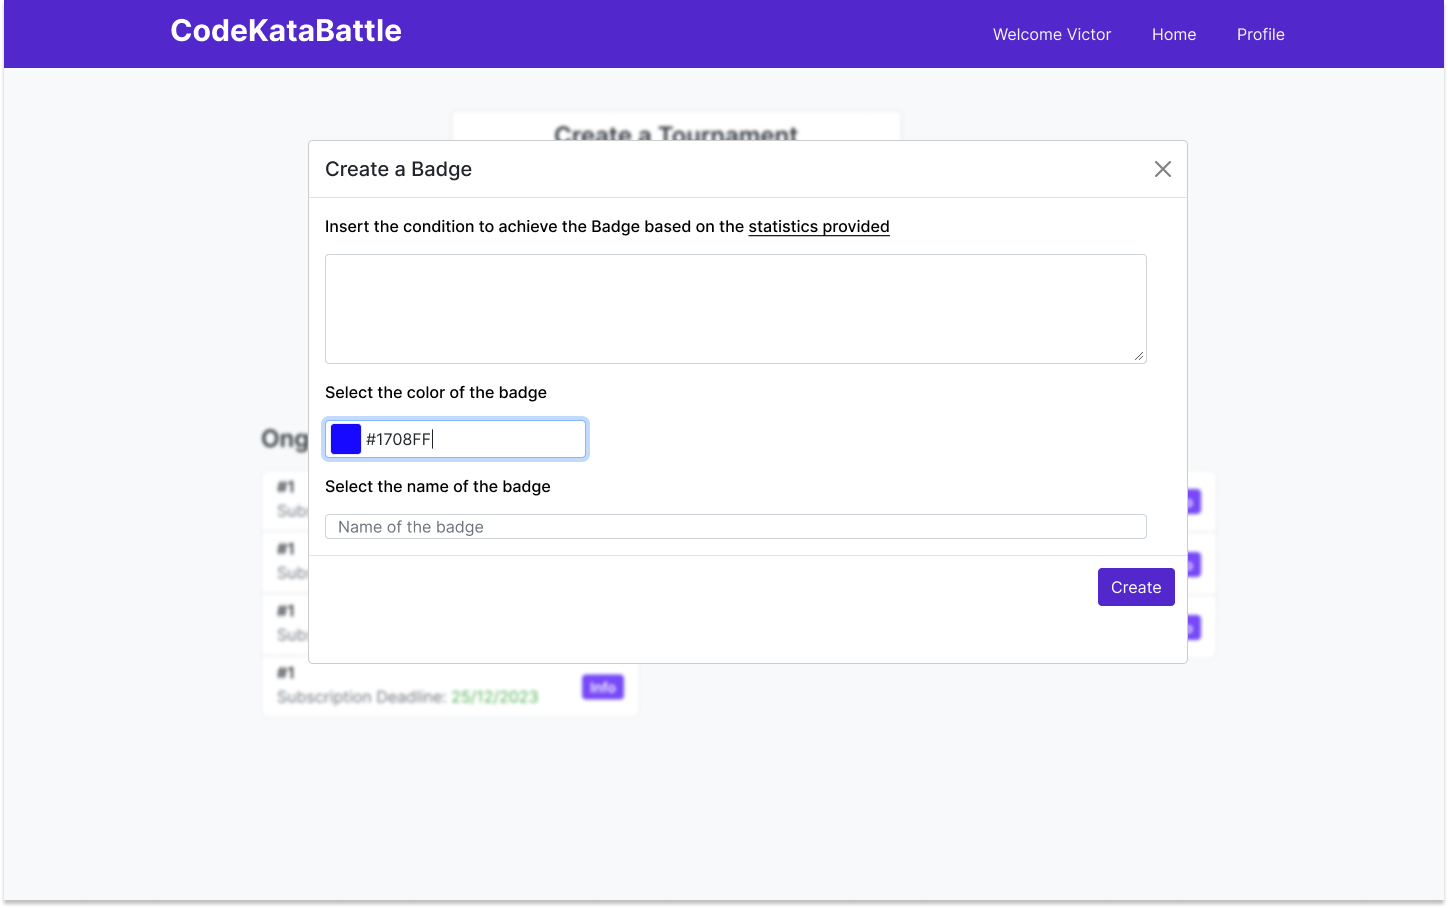
\includegraphics[scale = 0.25]{DD_latex/Images/UI/MainPageEducator-1.png}\\
\caption{Badge definition for a tournament (Educator)}
\end{figure}

\begin{figure}[H]
\centering
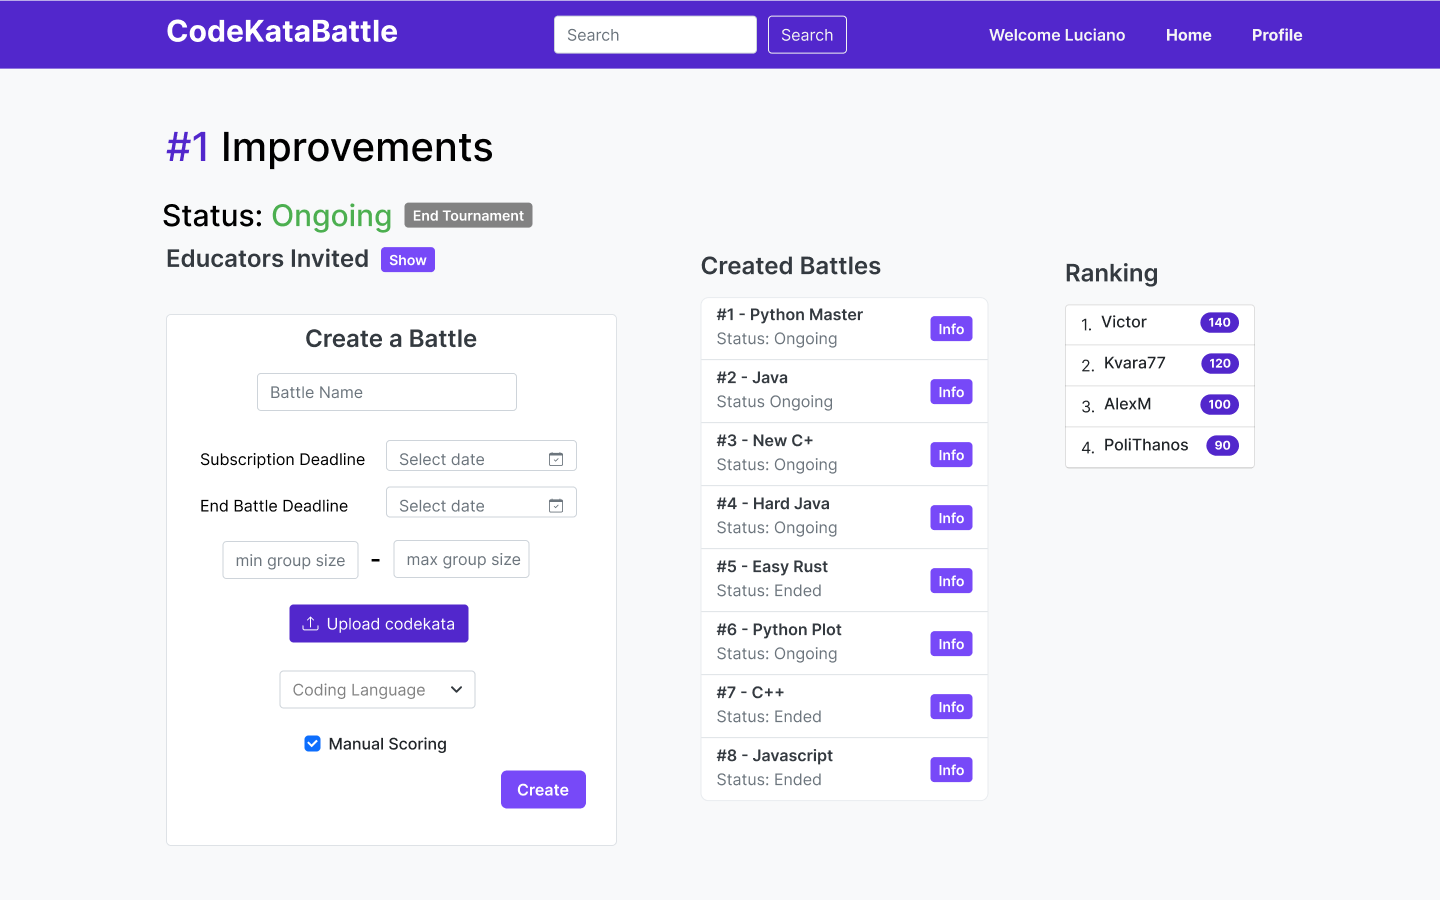
\includegraphics[scale = 0.25]{DD_latex/Images/UI/TournamentPage_EducatorCreator.png}\\
\caption{Tournament Page where the educator is the creator of the tournament (Educator)}
\end{figure}

\begin{figure}[H]
\centering
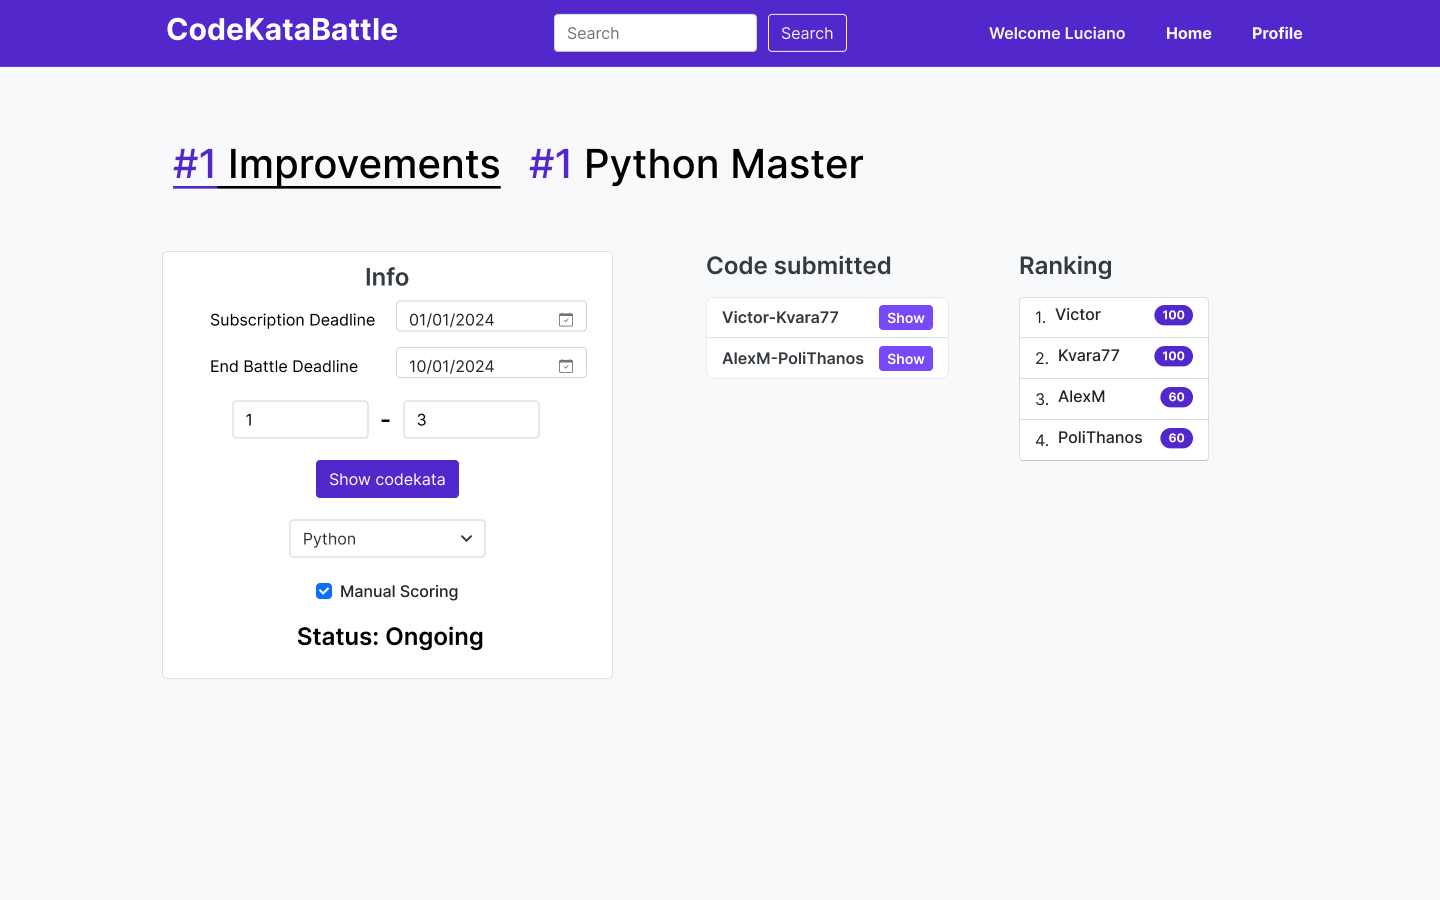
\includegraphics[scale = 0.25]{DD_latex/Images/UI/BattlePage_EducatorCreator.png}\\
\caption{Battle Page where the educator is the creator of the tournament (Educator)}
\end{figure}

{\color{bluepoli}\rule{\linewidth}{0.1pt}}

% FOURTH CHAPTER
% --------------------------------------------------------------------------
\chapter{Requirements Traceability}

% FIFTH CHAPTER
% --------------------------------------------------------------------------
\chapter{Implemenation, Integration and Testing Plan}

\section{Development Process and Approach}

{\color{bluepoli}\rule{\linewidth}{0.1pt}}

\section{Implementation Plan}

{\color{bluepoli}\rule{\linewidth}{0.1pt}}

\section{Integration Plan}

{\color{bluepoli}\rule{\linewidth}{0.1pt}}

\section{System Testing}

{\color{bluepoli}\rule{\linewidth}{0.1pt}}

% SIXTH CHAPTER
% --------------------------------------------------------------------------
\chapter{Effort Spent}

\section{Effort Spent per Unit}

This section shows the amount of time that each member has spent to produce the document. Please notice that each unit is the result of coordinated work among all the members.

\begin{table}[h]
\centering
\begin{tabularx}{\textwidth}{| X | X | X |}
\hline
\textbf{UNIT} & \textbf{MEMBERS} & \textbf{HOURS} \\ [1ex]
\hline
SetUp & Piccinato & 1h \\ [1ex]
\hline
\end{tabularx}
\end{table}

% SEVENTH CHAPTER
% --------------------------------------------------------------------------
\chapter{References}

\section{References and Tools}

\begin{enumerate}
    \item GitHub: https://www.github.com
    \item GitHub Actions: https://github.com/features/actions
    \item The UI Mockups have been made with: https://www.figma.com
\end{enumerate}

{\color{bluepoli}\rule{\linewidth}{0.1pt}}

\end{document}
